\section*{Q.2(a). \emph{$\delta$-wide Minimum Area Polygonization} (\dmap)}
Lets denote the problem by \emph{$\delta$-wide Minimum Area Polygonization} (\dmap). We consider the following assumptions:
\begin{multicols}{2}
	\begin{itemize}
		\item The machine tool enters and exits from the left boundary of sheet (any other case can be converted to this case using simple preprocessing)
		\item Points have integral, general coordinates.
		\item No two discs (defective points) overlap.
		\item $\delta \geq k$
		\item The tool cannot cut infitesimally small arcs (this allows us to ignore any curving and focus on polygonization).
	\end{itemize}
\end{multicols}
%\subsection{Hardness}
We first define the problem of \emph{Euclidean Steiner Tree} (\est) as follows: 
"Given $n$ terminal points in the plane, find the minimum length tree such that all $n$ terminals are conected and that any two terminal points may be interconnected by line segments either directly or via other points (called as steiner points) and line segments."

The problem \est is \NPH. Intuitively the \dmap can be reduced from \est by setting $k=0$ (consider the terminal points of \est as discs of \dmap) and $\delta = \eps$, where $\eps \approx 0$  (such that minimizing the area in \dmap becomes equivalent to minimizing the length of tree connecting the terminal points).


[Algorithm and Complexity]
\est has a PTAS (Polynomial Time Running Scheme) i.e. a $(1+\eps)$-approximation factor polynomial time algorithm \cite{byrka2010improved}. We use this PTAS as a black-box to obtain a near optimal solution for our problem. We call an edge a \emph{rail-road} if its a rectangular region with the almost the same length as that of edge ($\ell + k$) and a width of $\delta$ (its like a bloated edge along its width). Note that we also increase the length by $\frac{k}{2}$ to each side to cover the defective discs completely.
Intuitively we find a minimum steiner tree (MSNT) with edges as $\delta$-wide rail-roads. After obtaining the MSNT, we combine the leftmost point of MSNT to the left edge of sheet using a horizontal rail-road. The Algorithm; defined more formally; is given by \Cref{algo2a}.

\begin{algorithm}
\caption{PTAS \dmap (Run Shown in \Cref{fig:gen2})}\label{algo2a}
\begin{algorithmic}[1]
\STATE Run PTAS of \est with $n$ terminals as centres of $n$-defective spots to obtain MSNT \TT.
\STATE Find the leftmost point from the nodes of tree (maybe a non-terminal as well) say $p_{l}$.
\STATE Connect a horizontal edge from $p_{l}$ to left boundary of plane, call the corresponding point on boundary as $p_{b}$. 
\STATE Add the edge in previous step and $p_b$ to \TT (as shown in \Cref{fig:1}).
\STATE Replace the edge of \TT with rail-roads ($\delta$-wide rectangles of almost the same length as that of edge) such that the original edge passes through the centre of respective rail-road (i.e. partitioning it into two rectangles of same length but  $\frac{\delta}{2}$-width each) (as shown in \Cref{fig:2}).
\STATE Consider the $union^{refer~to~Techniques \& Data Structures}$ of region formed by rail-roads, say $\TT_{bloated}$ (clearly this is a polygon). Return $\TT_{bloated}$ as near-optimal solution to \dmap (as shown in \Cref{fig:3}).
\end {algorithmic}
\end{algorithm}

[Complexity] \Cref{algo2a} gives a PTAS i.e. $(1+\eps)$-approximation poly time algorithm for \dmap. Step 5 and 6 of algorithm take constant time (see Techniques $\&$ Data Structures). This is the best we can perform for a \NPH problem with a polynomial time algorithm. 

[Correctness]
Trivially, an optimal solution to \dmap must be a polygon with width no more (no less) than $\delta$ (if the width is greater than $\delta$ at some point, from our initial assumptions we can shrink the polygon at that place to get a smaller-area polygon). Since the width can be considered uniform (i.e. $=\delta$) throughout, the problem reduces to finding a minimum length tree than connects all the defective points (probably by using other points in the plane). Step 3 is justified as it appends a minimum area polygon/rail-road (minimum length edge) to the resulting tree. Again, since $\delta \geq k$ we can safely assume that the discs lie completely inside the returned polygon $\TT_{bloated}$.

[Techniques $\&$ Data Structures]\label{sec:tech}
 Apart from the PTAS-blackbox of \est, a major challenge while obtaining $\TT_{bloated}$ from $\TT$ is to compute union of convex polygons (i.e. rail-roads) obtained. We can do this by performing union of polygons considering two at a time. This can be done in constant time by doing triangulations of two polygons and then computing the Minkowski sum of each triangle obtained by a plane sweep algorithm which merges the boundaries of two polygons tracing out the new boundary (in general case it is $O(m+n)$, where $m$, $n$ are number of vertices of two polygons which is 4 each in our case).




\begin{figure}[H]
	\centering
	\subfigure[]{
		\resizebox{!}{4cm}{
			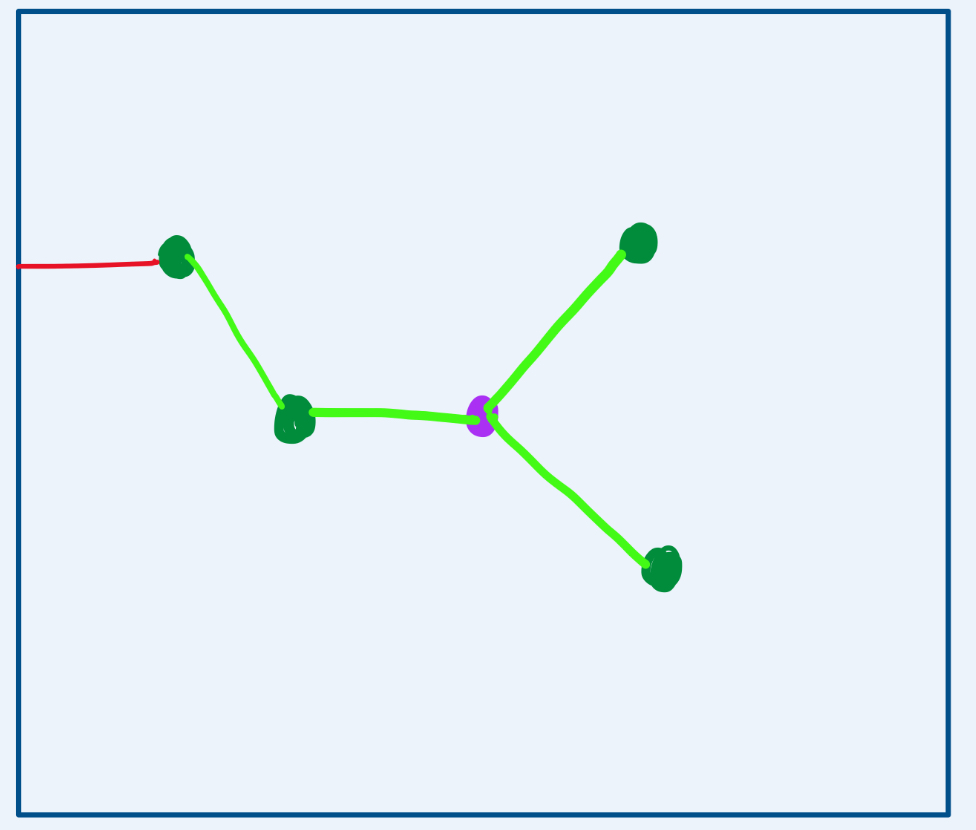
\includegraphics[scale=.1]{1.jpg}
			\label{fig:1}
		}
	}%\hspace{2cm}
	\subfigure[]{
		\resizebox{!}{4cm}{
			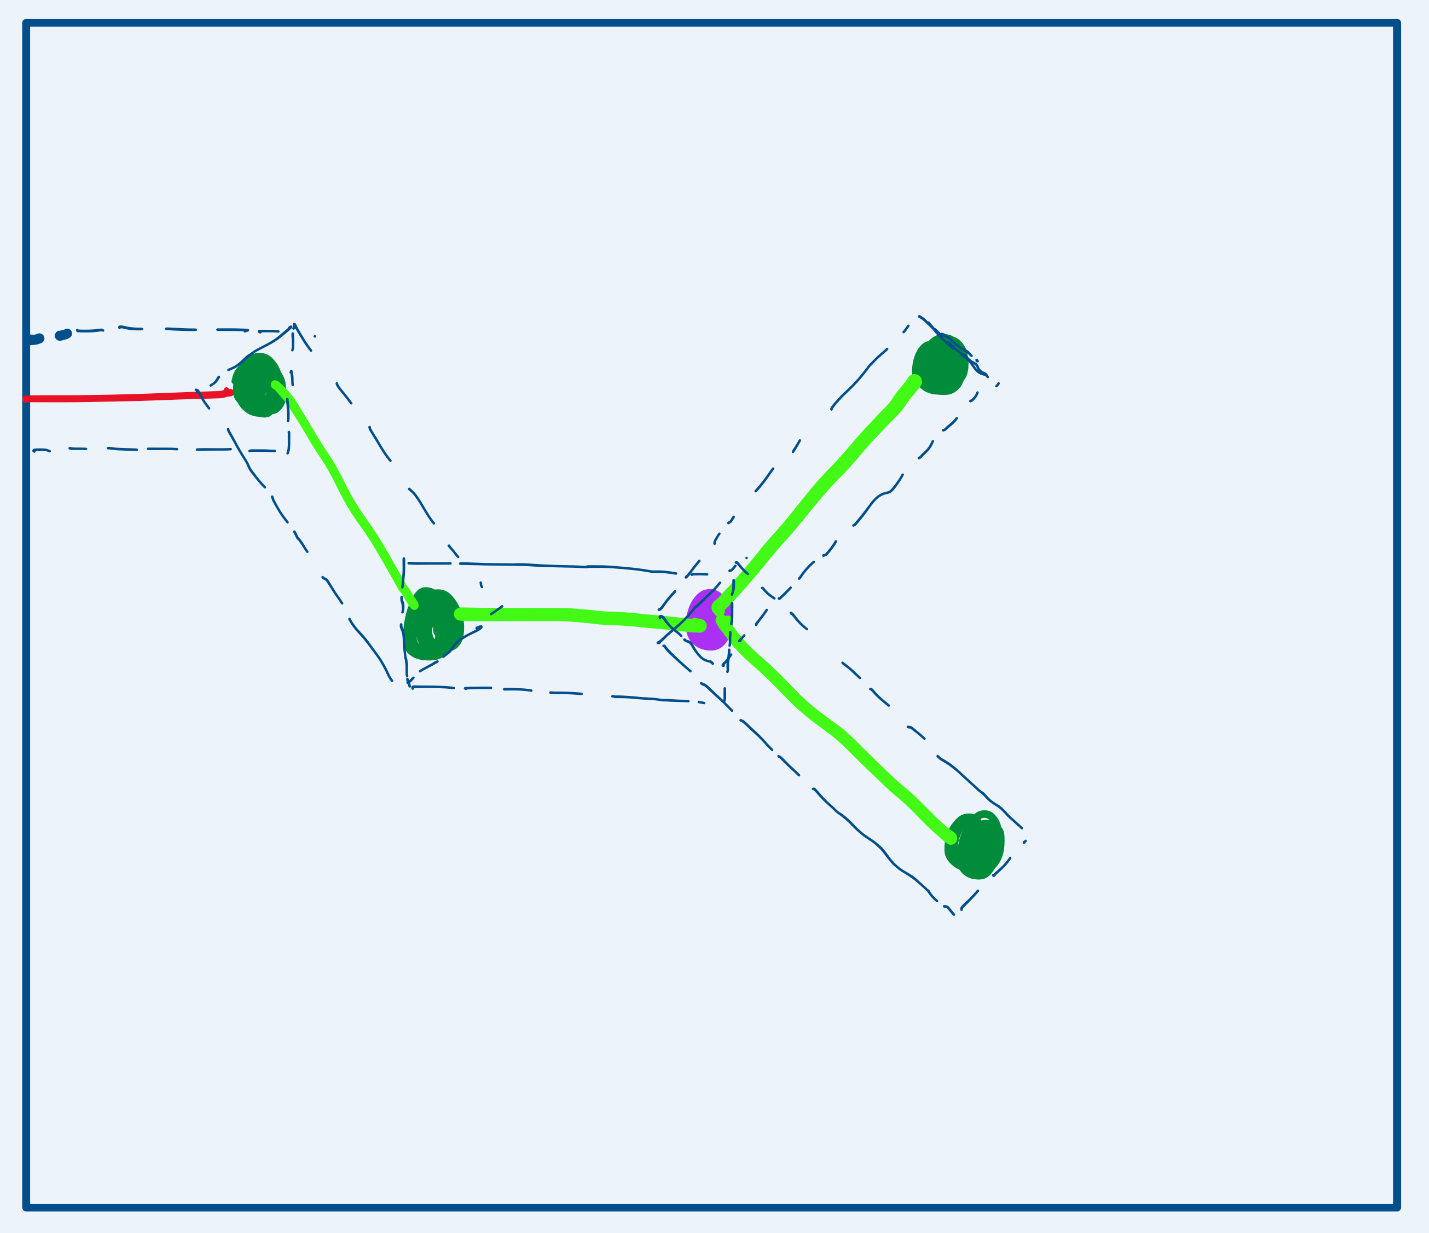
\includegraphics[scale=.1]{2.jpg}
			\label{fig:2}
		}
	}%\hspace{2cm}
	\subfigure[]{
		\resizebox{!}{4cm}{
			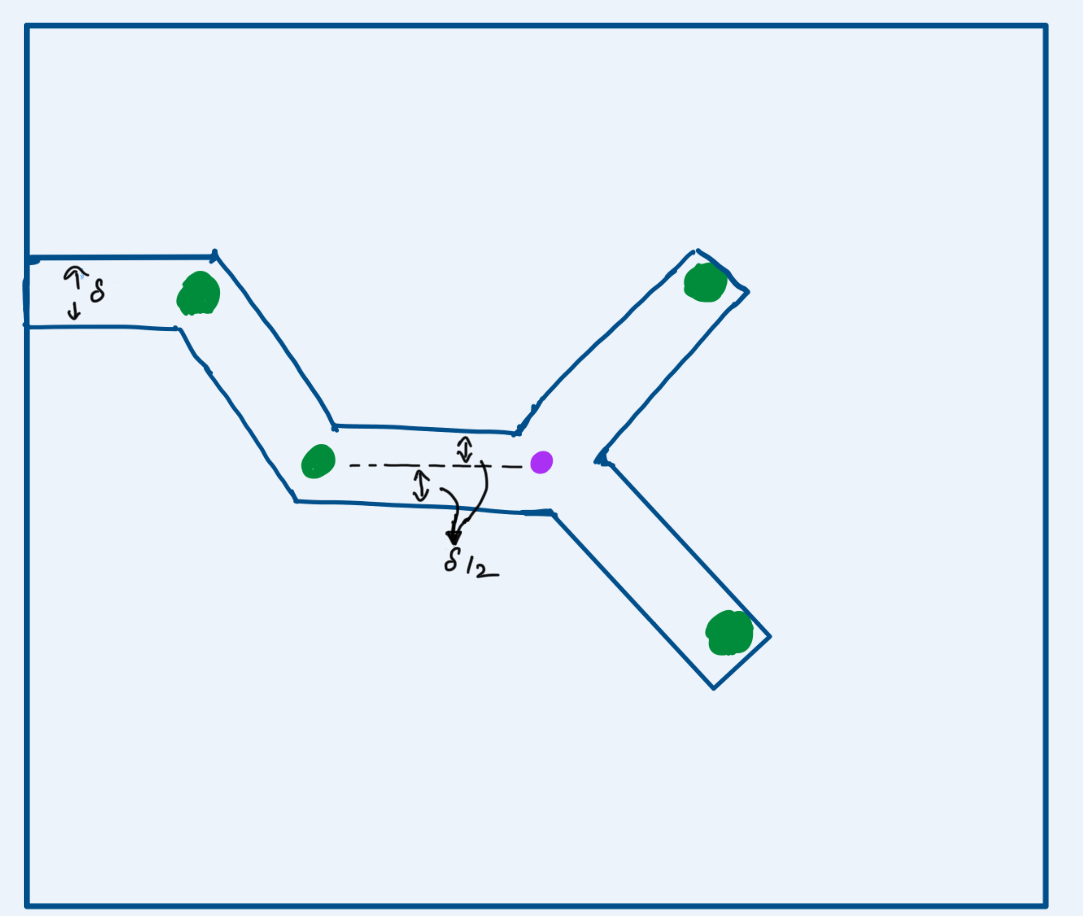
\includegraphics[scale=.1]{3.jpg}
			\label{fig:3}
		}
	}
	\caption{A Run of \Cref{algo2a}. (a) Step 1-4 : Defective Points (colored darkgreen), Steiner Point (colored purple), MSNT(Shown in light green) and an additional edge to leftmost point on tree(colored red). (b) Step 5: Replacing edges by $\delta$-wide rail-roads. (c) Step 6 : Merging the $\delta$-wide rail-roads to obtain $\TT_{bloated}$.}
	\label{fig:gen2}
\end{figure}


\pagebreak